% created on 2019-12-13
% @author : bmazoyer

%% Lines to compile only this capter
% \documentclass[11pt, twoside, a4paper, openright]{report}
% \usepackage[utf8]{inputenc}
% \DeclareUnicodeCharacter{223C}{~}

%Bibliography style
% \usepackage[square, numbers]{natbib}
% \usepackage[round]{natbib}
% \usepackage{biblatex}
% \bibliographystyle{unsrtnat}
% \bibliographystyle{unsrt}
% \bibliographystyle{plain}
% \bibliographystyle{aa}
% \usepackage[backend=bibtex,style=authoryear,natbib=true]{biblatex} 
\usepackage[
backend=biber,
style=authoryear,
citestyle=authoryear,
url=false
]{biblatex}
\addbibresource{../source/library.bib}

\usepackage[T1]{fontenc}
\usepackage[french]{babel}
\usepackage{csquotes}  % used for citations (recommended when using biblatex)
%\usepackage{helvet}
%\renewcommand{\familydefault}{\sfdefault}
\usepackage{mathptmx}
\usepackage{amssymb}
\usepackage{geometry} 
\usepackage{xcolor}
\usepackage[absolute,overlay]{textpos}
\usepackage{graphicx}
\usepackage{lipsum}
\usepackage[explicit]{titlesec}
\usepackage{lmodern}
\usepackage{color}
\usepackage{array}
\usepackage{mathtools}
\usepackage{caption}
\usepackage{multicol}
\usepackage{booktabs}
\usepackage{enumitem}
\usepackage{hyperref}
\usepackage{afterpage}
\usepackage{emptypage}
\usepackage{setspace}
\usepackage{pgffor}
    \setlength{\columnseprule}{0pt}
    \setlength\columnsep{10pt}
\usepackage[francais,nohints]{minitoc}
    \setcounter{minitocdepth}{3}
 
 %https://la-bibliotex.fr/2019/02/03/ecrire-les-nombres-et-les-unites-avec-latex/   
\usepackage{siunitx}
% \sisetup{
%     detect-all,
%      output-decimal-marker={,},
%      group-minimum-digits = 3,
%      group-separator={~},
%      number-unit-separator={~},
%      inter-unit-product={~},
%      list-separator = {, },
%      list-final-separator = { et },
%      range-phrase = --,
%      separate-uncertainty = true,
%      multi-part-units = single,
%      list-units = single,
%      range-units = single
%     }
\usepackage{physics}
\usepackage{isotope}

\usepackage[perpage]{footmisc} % to reset the counter of footnote each page

    
\usepackage{fancyhdr}			% Entête et pieds de page. Doit être placé APRES geometry
\pagestyle{fancy}		% Indique que le style de la page sera justement fancy
%\lfoot[\thepage]{} 		% gauche du pied de page
%\cfoot{} 			% milieu du pied de page
%\rfoot[]{\thepage} 
\fancyfoot{} % vide le pied~de~page
\fancyfoot[LE,RO]{\thepage}
\fancyfoot[LO,CE]{}% droite du pied de page
\fancyhead{}	
\fancyhead[LE]{\leftmark}	
\fancyhead[RO]{\rightmark}

\fancypagestyle{plain}{%
\fancyhf{} % vide l’en-tête et le pied~de~page.
\fancyfoot[LE,RO]{\thepage} % numéro de la page en cours en gras% et centré en pied~de~page.
\renewcommand{\headrulewidth}{0pt}
\renewcommand{\footrulewidth}{0pt}}



% Premiere page des chapitres
\newlength\chapnumb
\setlength\chapnumb{3cm}
 
\titleformat{\chapter}[block] {
  \normalfont}{}{0pt} { %police
    \parbox[b]{\chapnumb}{
      \fontsize{120}{110}\selectfont\thechapter} %taille du chiffre
      \parbox[b]{\dimexpr\textwidth-\chapnumb\relax}{
        \raggedleft 
        \hfill{\bfseries\Huge#1}\\ %taille du titre
        \rule{\dimexpr\textwidth-\chapnumb\relax}{0.4pt} %ligne de separation
  }
}
 
 %premiere page chapitre non numerote (remerciement, table des matieres ...)
 
\titleformat{name=\chapter,numberless}[block]
{\normalfont}{}{0pt}
{   
    \parbox[b]{\dimexpr\textwidth}{%   
    \hfill{\bfseries\Huge#1}\\
  \rule{\dimexpr\textwidth}{0.4pt}}}
    
 %   \titleformat{name=\chapter,numberless}[block]
%{\normalfont}{}{0pt}
%{\parbox[b]{\chapnumb}{%
%   \mbox{}}%
%  \parbox[b]{\dimexpr\textwidth-\chapnumb\relax}{%
%    \raggedleft%
%    \hfill{\bfseries\Huge#1}\\
%    \rule{\dimexpr\textwidth-\chapnumb\relax}{0.4pt}}}


%%%    SIunitx
\sisetup{locale = FR,
  % inter-unit-product=\ensuremath{\cdot},
  inter-unit-product=\ensuremath{\,},
  per-mode=reciprocal,
  separate-uncertainty = true,
  detect-all
}
\DeclareSIUnit{\Mpc}{Mpc}
\DeclareSIUnit{\kpc}{kpc}
\DeclareSIUnit{\Gpc}{Gpc}
\DeclareSIUnit{\h}{\textit{h}~}
\DeclareSIUnit{\perh}{\textit{h}^{-1}\,}

%%% Geometry
\geometry{
left=20mm,
top=30mm,
right=20mm,
bottom=30mm
}

%%% Color
\definecolor{bordeau}{rgb}{0.3515625,0,0.234375}

%%% Commands
\newcommand{\Nmocks}{\num{30}}
\newcommand{\hMpc}{h^{-1}\,\mathrm{Mpc}}
\newcommand{\hGpc}{h^{-1}\,\mathrm{Gpc}}
\newcommand{\kms}{\mathrm{km\,s^{-1}}}

\newcommand{\lya}{Ly$\alpha$}
\newcommand{\lyb}{Ly$\beta$}
\newcommand{\lyalya}{Ly$\alpha$(Ly$\alpha$)}
\newcommand{\lyalyb}{Ly$\alpha$(Ly$\beta$)}

\newcommand{\lrf}{\lambda_{\rm RF}}
\newcommand{\kpar}{k_{\parallel}}
\newcommand{\apar}{\alpha_{\parallel}}
\newcommand{\rpar}{r_{\parallel}}
\newcommand{\aperp}{\alpha_{\perp}}
\newcommand{\rperp}{r_{\perp}}
\newcommand{\kperp}{k_{\perp}}

\newcommand{\blya}{b_{\rm Ly\alpha}}
\newcommand{\betalya}{\beta_{\rm Ly\alpha}}
\newcommand{\blyb}{b_{\rm Ly\alpha}}
\newcommand{\betalyb}{\beta_{\rm Ly\beta}}
\newcommand{\dlya}{d_{\rm Ly\alpha}}
\newcommand{\bhcd}{b_{\rm HCD}}
\newcommand{\betahcd}{\beta_{\rm HCD}}
\newcommand{\Fhcd}{F_{\rm HCD}}
\newcommand{\Lhcd}{L_{\rm HCD}}

\newcommand{\imin}{i_{\rm min}}
\newcommand{\imax}{i_{\rm max}}
\newcommand{\jmin}{j_{\rm min}}
\newcommand{\jmax}{j_{\rm max}}

\newcommand{\xioned}{\xi_{\rm 1d}}
\newcommand{\DHub}{D_{H}}
\newcommand{\DM}{D_{M}}

\newcommand{\omegam}{\Omega_M}
\newcommand{\omegac}{\Omega_C}
\newcommand{\omegab}{\Omega_B}
\newcommand{\omegan}{\Omega_\nu}
\newcommand{\omegal}{\Omega_\Lambda}
\newcommand{\omegak}{\Omega_k}
\newcommand{\orad}{\Omega_R}
\newcommand{\ogam}{\Omega_\gamma}
\newcommand{\lcdm}{$\Lambda$CDM}

\newcommand{\picca}{\texttt{picca}}

%%% Rem's command
\newcommand\blankpage{%
    \null
    \thispagestyle{empty}%
    \addtocounter{page}{-1}%
    \newpage}
  
% Command to set up a particular alignment for a cell in tabular :
% \myalign{c}{foo} for instance
\newcommand*{\myalign}[2]{\multicolumn{1}{#1}{#2}}
 
\renewcommand{\thesection}{\arabic{section}}

% Romain
\newcommand{\cRM}[1]{\MakeUppercase{\romannumeral #1}}	% Capital
\newcommand{\cRm}[1]{\textsc{\romannumeral #1}}	% Petit majuscule
\newcommand{\crm}[1]{\romannumeral #1}
% Siècle %
\newcommand{\siecle}[1]{\cRm{#1}\textsuperscript{e}~siècle}



% Thesis title
\newcommand{\PhDTitle}{Les forêts \lya{} du relevé eBOSS : comprendre les fonctions de corrélation et les systématiques} 

% Name
\newcommand{\PhDname}{Thomas Etourneau} 

% Change this variable if you add or remove chapters
\newcommand*{\NumOfChapters}{6}

% Change this variable if you add or remove appendices
\newcommand*{\NumOfAppendices}{2}

% PDF metadata
\hypersetup{
	pdfauthor={\PhDname},
	pdfsubject={Manuscrit de thèse de doctorat},
	pdftitle={\PhDTitle}
}


% \begin{document}
%%

\graphicspath{ {../figures/donnees/} }

\chapter{Présentation des données}
\minitoc
\newpage
\thispagestyle{fancy}

Dans le chapitre précédent, nous présentions l'instrument SDSS et le relevé eBOSS.
% Nous présentons ici, comment des photons acquis avec les CCD, les spectres sont déduits, puis comment du spectre de chaque quasar, le champ d'absortion est reconstruit.
Nous présentons ici comment les spectres sont déduits des photons acquis par les CCD, puis comment le spectre d'absorption est reconstruit à partir de chaque spectre.

\section{Réduction des données}
\label{sec:reduction_donnees}
L'observation de chaque plaque fournit des données en deux dimensions : la première correspond aux différentes longueurs d'onde, la seconde aux différentes fibres (voir figure~\ref{fig:photo_ccd}). La chaîne de réduction des données transforme ces informations en une liste de spectres.
Premièrement, chaque spectre est extrait de l'image acquise par le CCD. Le spectre est étalonné en longueur d'onde à l'aide de lampes à arc. Le flux est calibré en utilisant les spectres des fibres dédiées à des étoiles standards.
Puis le fond du ciel, estimé dans chaque demi-plaque grâce aux fibres dédiées, est soustrait à chaque spectre.
La variance dans chaque pixel est ensuite estimée. Elle prend en compte le bruit de photon et le bruit de l'électronique. Les pixels affectés par des rayons cosmiques sont rejetés.
Enfin, pour chaque objet, toutes les expositions sont ajoutées pour former un seul et même spectre, avec un plus grand rapport signal sur bruit. Le nombre typique d'expositions par objet varie entre 4 et 6.

\paragraph{}
Les données que nous utilisons dans ce manuscript ont été rendues publiques lors de la seixième publication de données SDSS (DR16\footnote{https://www.sdss.org/dr16/}). Elles sont décrites par \textcite{Ahumada2019}.
\begin{figure}[b]
  \centering
  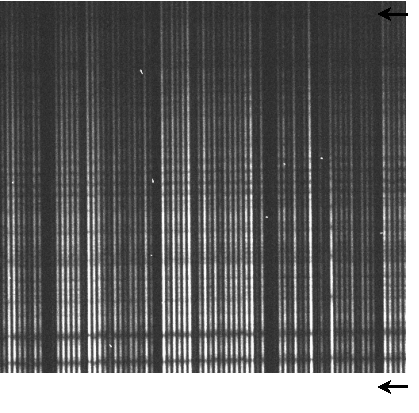
\includegraphics[scale=0.8]{photo_ccd.pdf}
  \caption{Photographie d'un capteur CCD. L'axe des absysses indique le numéro de la fibre optique. L'axe des ordonnées donne la longueur d'onde observée.}
  \label{fig:photo_ccd}
\end{figure}

\section{Le catalogue de quasar}
Une fois les spectres extraits, il est important de les classifier afin de construire des catalogues utilisables par les différentes analyses. Pour ce faire, chaque spectre est traité par le pipeline de SDSS, décrit par \textcite{Bolton2012}.
% A chaque spectre est ajusté plusieurs modèles d'étoiles, de galaxies et de quasars. Les modèles sont construits en utilisant les \emph{PCA templates} : des spectres typiques qui sont combinés afin d'ajuster au mieux le spectre à classifier.
\textbf{Plusieurs modèles d'étoiles, de galaxies et de quasars sont ajustés à chaque spectre.
%   Ces modèles sont construits à l'aide de l'analyse en composantes principales (PCA). Cette analyse fournit des spectres typiques de complexités différentes, le moins complexe étant la moyenne. Les différents spectres sont alors pondérés et combinés afin de construire un modèle qui ajuste au mieux le spectre à classifier.}
Chaque modèle est construit à l'aide d'une analyse en composantes principales (PCA), propre à chaque type d'objet. Pour chaque type d'objet, l'analyse fournit des spectres typiques. Ces derniers sont de complexités croissantes : le premier donne le plus d'information comme par exemple le spectre moyen, les spectres plus complexes donnent des détails comme certaines raies d'émission ou profile d'absorption. Ces spectres typiques sont pondérés et combinés afin de produire un spectre simulé qui ajuste aux mieux le spectre à classifier.}
Une fois tous les modèles ajustés, ils sont triés selon leur $\chi^{2}$ réduit. Le spectre est alors classifié selon le modèle possédant le plus faible $\chi^{2}$ réduit.
Tous les spectres mesurés par SDSS et classifiés comme quasar constituent l'échantillon \emph{superset}. Il contient \num{1440627} objets.

Certains quasars peuvent être difficiles à classifier à cause d'absorptions intenses comme les DLA ou les BAL\footnote{Les BAL (Broad Absorption Line) sont des quasars qui présentent des absorptions intenses au voisinage de leurs raies d'émission. Cette absorption est interprétée comme étant due à un absorbeur dense situé juste devant le quasar. La figure~\ref{fig:exemple_bal} présente un spectre de quasar avec un BAL.}.
Tous les quasars du relevé BOSS ont été inspectés visuellement \autocite{Paris2016} afin de confirmer la classification du pipeline de SDSS, et d'estimer leur redshifts. Cet échantillon représente \num{297301} objets.
\begin{figure}
  \centering
  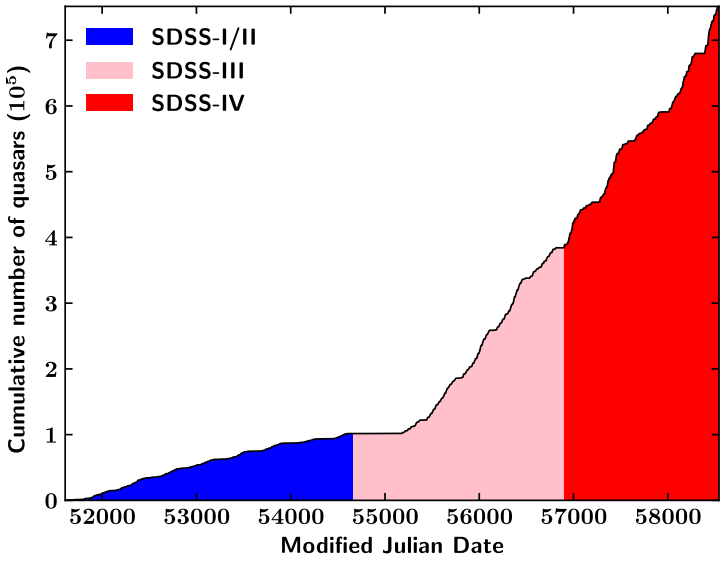
\includegraphics[scale=0.35]{quasar_number}
  \caption{Evolution du nombre de quasars observés par les différentes générations de SDSS en fonction du temps. Les générations SDSS I et II correspondent à $MJD < 54663$ (bleu), SDSS III à $54663 \leq MJD < 56898$ (rose) et SDSS IV à $56898 < MJD < 58543$ (rouge). Crédits : \textcite{Lyke2019}}
  \label{fig:quasar_number}
\end{figure}
\begin{figure}
  \centering
  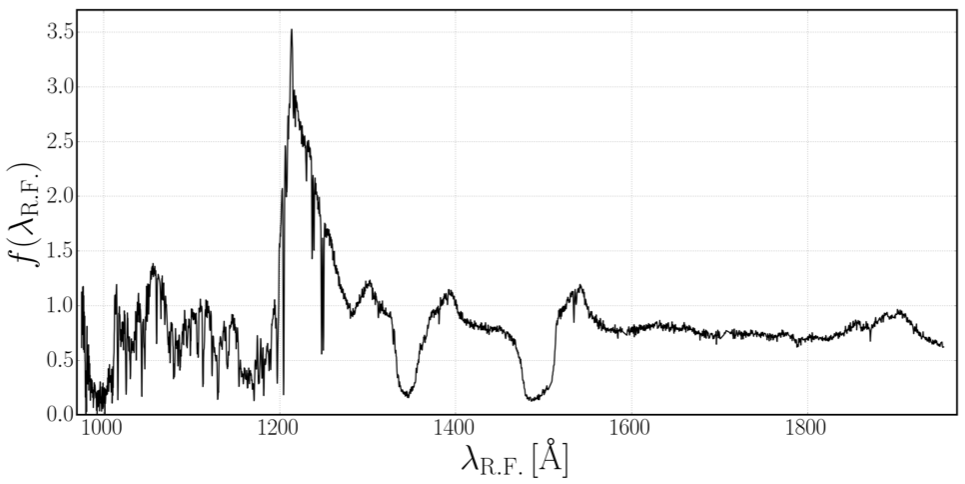
\includegraphics[scale=0.4]{exemple_bal}
  \caption{Spectre d'un quasar pris par SDSS présentant un BAL. Le spectre est très fortement absorbé pour les longueurs d'onde légèrement inférieures à chaque raie d'émission.}
  \label{fig:exemple_bal}
\end{figure}
Cependant, à cause du grand nombre de quasars observés par eBOSS (voir figure~\ref{fig:quasar_number}), l'observation visuelle n'a pas pu être effectuée pour tous ces objets.
% Une deuxième classification, fondée sur le pipeline de SDSS, est alors appliquée \autocite{CITE:Lyke in prep}.
% Elle est complétée par l'algorithme \texttt{QuasarNET} \autocite{Busca2018} afin de réduire le nombre de mauvaises et non-identifications, et donc le nombre d'inspections visuelles nécessaires. Grâce à \texttt{QuasarNET}, ce chiffre est réduit à \SI{0.6}{\percent} des spectres, soit \num{8581} spectres. Une sous-échantillon du superset est alors construit. Il contient \num{750426} objets, confirmés comme quasar par la chaîne de traitement précédente.
Afin de vérifier la première identification faite par le pipeline de SDSS, une seconde classification est alors effectuée \autocite{Lyke2019}. Elle est complétée par l'algorithme \texttt{QuasarNET} \autocite{Busca2018}. Ceci réduit le nombre d'identifications douteuses et donc le nombre d'inspections visuelles requises. A la fin, \SI{0.6}{\percent} des spectres, soit \num{8581} spectres, requièrent une inspection visuelle.

Une fois les spectres classifiés, un sous-échantillon du superset est construit. Il contient \num{750426} objets, confirmés comme quasar par la chaîne de traitement précédente.
Pour chaque objet, le catalogue fournit plusieurs estimations de redshift. Le pipeline de SDSS produit une première estimation. L'algorithme \texttt{QuasarNET} en fournit une seconde. Les spectres inspectés visuellement possèdent une autre estimation. Enfin, l'algorithme \texttt{redvsblue}\footnote{https://github.com/londumas/redvsblue} produit plusieurs estimations de redshift, parmi lesquelles figurent \texttt{Z\_PCA} et \texttt{Z\_LYAWG}.

Différents algorithmes sont alors appliqués au catalogue, afin d'identifier les DLA et les BAL présents. L'identification utilise l'addition des différentes expositions pour chaque objet.
Concernant les DLA, l'algorithme de détection est décrit dans \textcite{Parks2017}. Il est appliqué sur les quasars à un redshift $2 \leq \texttt{Z\_PCA} \leq 6$, afin d'avoir suffisamment de pixels dans la zone $900 < \lambda_{\mathrm{RF}} < \SI{1346}{\angstrom}$. Parmi les \num{270315} spectres inspectés, \num{39514} DLA ont été identifiés, distribués dans \num{35686} spectres.
Concernant les BAL, l'algorithme utilisé est très similaire à celui décrit dans \textcite{Guo2019}. Les BAL sont recherchés dans les spectres ayant un redshift entre \num{1.57} et \num{5.6}. L'algorithme fournit la probabilité qu'un spectre possède un BAL. Le champ \texttt{BAL\_PROB} du catalogue indique cette probabilité.

A la fin, le catalogue ainsi construit (DR16Q dans la suite de ce manuscrit) contient \num{750426} quasars confirmés. Nous référons le lecteur à l'article \textcite{Lyke2019} pour davantage d'informations.



\paragraph{}
L'analyse \lya{} des données complètes d'eBOSS \autocite{DuMasdesBourboux2020} utilise le catalogue DR16Q. Le redshift des quasars est choisi comme étant \texttt{Z\_LYAWG}. Les quasars sont sélectionnés avec un redshift $\num{1.77} < z \leq 4$. L'échantillon correspondant représente alors \num{341468} objets. La distribution en redshift de ces quasars traceurs (ceux utilisés comme traceurs pour la fonction de corrélation croisée \lya{}-QSO) est présentée dans le graphique de gauche de la figure~\ref{fig:pixel_number}.
\begin{figure}
  \centering
  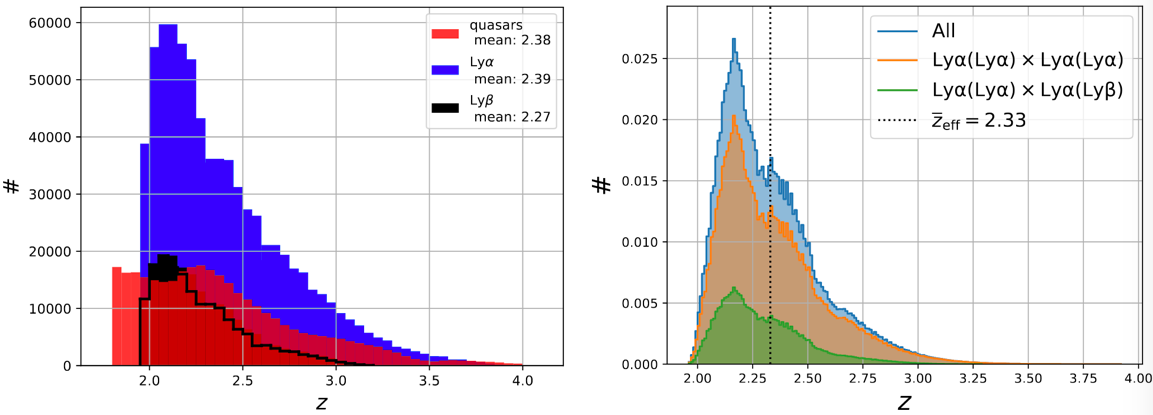
\includegraphics[scale=0.4]{pixel_number}
  \caption{Gauche : distribution en redshift des pixels \lyalya{} (bleu) et des pixels\lyalyb{} (noir) (nombres divisés par 50), ainsi que celle des quasars traceurs (rouge). Droite : distribution pondérée du redshift efficace de chaque paire de pixels utilisée pour le calcul de la fonction corrélation du \lya{}. La distibution orange présente les paires de pixels \lyalya{}-\lyalya{}, la verte les paires de pixels \lyalya{}-\lyalyb{}, et la bleu la somme des deux. Les paires représentés sont celles nécessaires pour la mesure de la position du pic BAO, c'est à dire avec une séparation $r \in [\num{80} \,; \num{120}] \si{\perh\Mpc}$. La ligne en pointillés indique le redshift effectif de la mesure, c'est à dire la moyenne de la distribution bleue. Il vaut $z_{eff} = \num{2.334}$.}
  \label{fig:pixel_number}
\end{figure}


\section{La sélection des forêts}
\label{sec:selection_forets}
L'analyse \lya{} des données complètes d'eBOSS, dont nous nous servons dans ce manuscrit, est présentée dans l'article \textcite{DuMasdesBourboux2020}. Les informations que nous donnons dans la suite de ce chapitre sont tirés de cette article. Nous y référons le lecteur pour davantage d'informations.

Les spectres produits par la chaîne de réduction des données SDSS sont rebinnés : 3 pixels du spectre original, d'une taille $\Delta log_{10}(\lambda) \sim 10^{-4}$, sont combinés en 1 seul pixel d'analyse, d'une taille $\Delta log_{10}(\lambda) \sim 3 \times 10^{-4}$. Ceci est fait afin de réduire le temps de calcul nécessaire pour estimer les fonctions de corrélation. Dans la suite, l'utilisation de ``pixel'' réfère à ces pixels d'analyse.

L'absorption \lya{} est mesurée dans deux régions disctinctes du spectre. La première, dénommée région \lya{}, correspond aux longueurs d'onde $\num{1040} \leq \lambda_{\mathrm{RF}} \leq \SI{1200}{\angstrom}$, c'est à dire entre les raies d'émission \lyb{} et \lya{}. La seconde, dénommée région \lyb{}, correspond aux longueurs d'onde $\num{920} \leq \lambda_{\mathrm{RF}} \leq \SI{1020}{\angstrom}$, c'est à dire entre la limite de la série de Lyman et la raie d'émission \lyb{}. Les pixels d'absorption \lya{} dans la région \lya{} sont dénommés pixels \lyalya{}, et ceux dans la région \lyb{} sont dénommés pixels \lyalyb{}.
De plus, l'analyse se limite aux pixels dont la longueur d'onde observée est comprise entre $\num{3600} \leq \lambda_{\mathrm{obs}} \leq \SI{6000}{\angstrom}$.
La limite inférieure provient de la sensibilité des CCD et de l'augmentation des absorptions atmosphériques intenses dans l'UV. La limite supérieure provient des raies d'émission du ciel dans le proche infrarouge qui bruitent le signal.
% à cause notamment des absorptions atmosphériques intenses dans l'UV, et des raies d'émissions du ciel dans le proche infrarouge.
% Ces limites sur $\lambda_{\mathrm{obs}}$ correspondent à un redshift minimal $z_{\textsc{QSO}} = 2$ pour les quasars \lya{}, et $z_{\textsc{QSO}} = 2.53$ pour les quasars \lyb{}. Parmi les \num{341468} quasars utilisés \textbf{comme traceurs pour la corrélation croisée \lya{}-\textsc{QSO}} (dénommés quasars traceurs), \num{256328} sont utilisés pour leurs pixels \lyalya{} (dénommés quasar \lya{}), et \num{103080} sont utilisés pour leurs pixels \lyalyb{} (dénommés quasar \lyb{}).
Ces limites sur $\lambda_{\mathrm{obs}}$ correspondent à un redshift minimal $z_{\textsc{QSO}} = 2$ pour les quasars utilisés pour leurs pixels dans la région \lya{} (quasars \lya{}), et $z_{\textsc{QSO}} = \num{2.53}$ pour les quasars utilisés pour leurs pixels dans la région \lyb{} (quasars \lyb{}). Parmi les \num{341468} quasars traceurs, \num{256328} sont des quasars \lya{}, et \num{103080} sont des quasars \lyb{}.

D'autres sélections sont aussi appliquées. Les quasars pour lesquels la probabilité d'avoir un BAL est supérieure à 0.9 sont écartés. Les mauvaises observations durant BOSS ou eBOSS sont mises de côté. De plus, chaque région nécessite au moins 50 pixels. Cette sélection décale le redshift minimal à $z_{\textsc{QSO}} = \num{2.10}$ pour les quasars \lya{}, et à $z = \num{2.65}$ pour les quasars \lyb{}. Le pixel d'absorption \lya{} de plus bas redshift se trouve à $z = \num{1.96}$. Enfin, l'ajustement du continuum (voir section suivante) échoue pour environ \SI{2}{\percent} des spectres). Ces spectres sont aussi écartés.
Après toutes ces sélections, l'échantillon final contient \num{210005} quasars \lya{} et \num{69656} quasars \lyb{}. 
% La distribution en redshift des pixels et des quasars traceurs est présentée dans le graphique de gauche de la figure~\ref{fig:pixel_number}.

Enfin, des corrections sur le flux et la variance du flux sont appliquées afin de corriger les imperfections de la chaîne de réduction. De plus, certaines régions spectrales en longueur d'onde observée sont masquées, à cause de l'augmentation de la variance du flux causée par les raies du ciel. Tout ceci est décrit en détail dans \textcite{DuMasdesBourboux2020}.

\section{Définition du champ d'absorption}
Dans cette section, nous décrivons comment, du flux mesuré $f_q(\lambda)$ du quasar $q$ à la longueur d'onde observée $\lambda$, nous pouvons déduire les fluctuations du champ d'absorption \lya{}.
La démarche que nous décrivons ici est très bien expliquée dans la thèse \textcite{DeSainteAgathe}. Nous y référons le lecteur pour plus de détails.

\subsection{Calcul des $\delta$}
\label{subsec:calcul_delta}
Comme présenté dans la section~\ref{subsec:lya}, le contraste de l'absorption \lya{} $\delta_q(\lambda)$ est défini comme
\begin{equation}
  \label{eq:deltaF}
  \delta_q(\lambda) = \frac{f_q(\lambda)}{\overline F(\lambda) C_q(\lambda)} - 1 \;,
\end{equation}
où $\overline F(\lambda)$ est la transmission moyenne au redshift $z = \lambda / \lambda_{\mathrm{Ly}\alpha} - 1$, et $C_q(\lambda)$ donne le flux du spectre sans absorption. Il est dénommé \emph{continuum} et est différent pour chaque quasar.
Le produit $\overline F(\lambda) C_q(\lambda)$ représente donc le flux moyen attendu du quasar $q$.
La figure~\ref{fig:foret_lya} représente ces quantités pour les régions \lya{} et \lyb{}.
Du fait de la faible résolution et du faible rapport signal sur bruit des données, $\overline F(\lambda)$ n'est pas mesurable. Pour ne pas dépendre d'analyses externes, on détermine directement le produit $\overline F(\lambda) C_q(\lambda)$ pour chaque spectre.
Afin de prendre en compte la variabilité d'un spectre à un autre, le produit $\overline F(\lambda) C_q(\lambda)$ est modélisé par une relation linéaire en $\mathrm{log}_{10} \lambda$ :
\begin{equation}
  \label{eq:diversity}
  \overline F(\lambda) C_q(\lambda) = \overline C(\lambda_{\mathrm{RF}})(a_q + b_q \log_{10}(\lambda)) \; ,
\end{equation}
où $\overline C(\lambda_{\mathrm{RF}})$ donne le continuum moyenné sur tous les spectres, en fonction de la longueur d'onde dans le référentiel du quasar. $a_q$ et $b_q$ sont propres à chaque quasar, ils modélisent la diversité des quasars.
Les termes $a_q$, $b_q$ et $\overline C(\lambda_{\mathrm{RF}})$ sont déterminés en minimisant la fonction de vraissemblance $L$, qui s'exprime comme
\begin{equation}
  \label{eq:likelihood}
  - 2 \ln L = \sum\limits_{i} \frac{\left[f_{i} - \overline F C_q(\lambda_{i}, a_q, b_q)\right]^2}{\sigma_q^2 (\lambda_i)} + \ln [\sigma_q^2 (\lambda_i)] \;  .
\end{equation}
La variance $\sigma_q^2(\lambda)$ dans chaque pixel est donnée par
\begin{equation}
  \label{eq:variance}
  \sigma_q^2(\lambda) = \eta(\lambda) \sigma_{\mathrm{instru}, q}^2(\lambda) + \sigma_{\mathrm{cosmo}}^2 (\lambda) (\overline F C_q(\lambda))^2 + \frac{\epsilon(\lambda)(\overline F C(\lambda))^4}{\sigma_{\mathrm{instru},q}^2 (\lambda)}  \; .
\end{equation}
Le terme $\eta(\lambda)\sigma_{\mathrm{instru}, q}^2(\lambda)$ rend compte de la variance qui est provoquée par l'instrument et liée à l'incertitude sur la mesure des flux. Le terme $\sigma_{\mathrm{cosmo}}(\lambda)$ est purement cosmologique et donne la variance propre au champ d'absorption du \lya{}. Il traduit le fait que certaines régions de l'univers peuvent absorber plus ou moins que la moyenne. Du fait de l'isotropie, $\sigma_{\mathrm{cosmo}}$ ne dépend que de $z$. Le terme ad hoc $\epsilon(\lambda)(\overline F C(\lambda))^4 / \sigma_{\mathrm{instru},q}^2 (\lambda)$ rend compte du fait que la variance augmente avec le rapport signal sur bruit, probablement à cause de la diversité des quasars.
% \textbf{Enfin, le terme $\ln (\sigma_q^2)$ dans l'expression de la vraissemblance provient du fait que les erreurs $\sigma_q$ utilisées dans la détermination de $a_q$, $b_q$ et $\overline C(\lambda_{\mathrm{RF}})$ ne sont pas constantes et dépendent elles mêmes de ces paramètres.}
\textbf{Enfin, le terme $\ln [\sigma_q^2]$ dans l'expression de la vraissemblance provient de la normalisation $\sqrt{2 \pi \sigma^2}$ au dénominateur des distributions gaussiennes. Ce terme est généralement omis car constant. Mais dans notre cas, $\sigma_q$ dépend de $a_q$, $b_q$ et $\overline C(\lambda_{\mathrm{RF}})$.
}

Afin d'obtenir le produit $\overline F C_q$ pour chaque quasar, il faut maximiser la fonction de vraissemblance $L$ (équation~\ref{eq:likelihood}), et donc ajuster les paramètres $a_q$, $b_q$, $\eta(\lambda)$, $\sigma_{\mathrm{cosmo}}(\lambda)$ et $\epsilon(\lambda)$. Cependant, celle fonction dépend elle même du produit $\overline F C_q$. Pour résoudre ce problème, l'ajustement est fait de manière itérative.
Premièrement, les 5 paramètres à ajuster, ainsi que $\overline C(\lambda_{\mathrm{RF}})$, sont initialisés. Ceci permet d'ajuser $\overline F C_q$ sur $f_q(\lambda)$ en maximisant la fonction de vraissemblance $L$. Dans cet ajustement, chaque pixel observé à une longueur d'onde $\lambda$ est pondéré par un poids
\begin{equation}
  \label{eq:weights}
  w_{q}(\lambda) = \frac{1}{\sigma_{q}^2(\lambda)}  \; .
\end{equation}
Une fois cette ajustement fait, $\overline C(\lambda_{\mathrm{RF}})$ est de nouveau calculé. Puis, les paramètres $\eta(\lambda)$, $\sigma_{\mathrm{cosmo}}(\lambda)$ et $\epsilon(\lambda)$ sont ajustés de manière à ce que, à lambda fixé, $\sigma_q(\lambda)$ reproduise la variance estimée à partir des flux $f_q(\lambda)$ de tous les quasars. Ce nouvel ajustement permet une nouvelle fois d'ajuster $\overline F C_q$, etc. Cette procédure est répétée jusqu'à obtenir des valeurs stables pour les paramètres ajustés. En pratique, 5 itérations sont nécessaires.
Cette procédure permet donc d'estimer, pour chaque quasar, le produit $\overline F(\lambda) C_q(\lambda)$, et ainsi d'estimer les $\delta_q(\lambda)$ (équation~\ref{eq:deltaF}) indépendamment dans chaque région.

\textbf{Lors du calcul des $\delta_q$, les DLA identifiés dans chaque forêt sont masqués. Pour ce faire, un profil de Voigt, dépendant de la densité de colonne mesurée par l'algorithme de détection, est ajusté à l'endroit du spectre où le DLA a été identifié. Les pixels pour lesquels l'absorption est plus grande que \SI{20}{\percent} ne sont pas utilisés. Les autres sont corrigés en utilisant le profile de Voigt ajusté. La figure~\ref{fig:exemple_dla} montre deux spectres présentant un DLA. Le profile de Voigt est montré en dessous de la forêt, en rouge. Les bandes rouges indiquent les pixels non utilisés.}


\subsection{Prise en compte de l'ajustement du continuum}
\label{subsec:projdelta}
La procédure décrite dans la section précédente permet d'ajuster le continuum de chaque quasar afin d'estimer le champ $\delta$ dans chaque région d'absorption \lya{}. Cependant, cet ajustement biaise le champ $\delta$ mesuré, et introduit de fausses corrélations lors du calcul des fonctions de corrélation. Il est donc important de prendre en compte cet effet.
% Dans la suite, $\delta_q$ dénote le champ original, et $\tilde \delta_q$ le champ estimé.
% La modélisation de la diversité des quasars avec les paramètres $a_q$ et $b_q$ (équation~\ref{eq:diversity}) force la moyenne et la pente des $\\tilde delta_q$ à zéro. 

En redéfinissant les paramètres $a_q$ et $b_q$, l'équation~\ref{eq:diversity} peut être mise sous la forme
\begin{equation}
  \label{eq:diversity2}
  \overline F(\lambda) C_q(\lambda) = \overline C(\lambda_{\mathrm{RF}})(a_q + b_q (\Lambda - \overline \Lambda_q))  \; ,
\end{equation}
où $\Lambda = \log_{10} \lambda$, et $\overline \Lambda_q$ est la moyenne de $\Lambda$ dans chaque forêt :
\begin{equation}
  \label{eq:lambda_mean}
  \overline \Lambda_q = \frac{\sum\limits_{\lambda} w_q(\lambda) \Lambda}{\sum\limits_{\lambda} w_q(\lambda)}  \; .
\end{equation}
Le champ $ \delta_q$ mesuré est donc donné par
\begin{equation}
  \label{eq:deltaF2}
   \delta_q(\lambda) = \frac{f_q(\lambda)}{\overline C(\lambda_{\mathrm{RF}})(a_q + b_q (\Lambda - \overline \Lambda_q))} - 1  \; .
\end{equation}
Du fait que $a_q$ et $b_q$ sont ajustés sur les $f_q(\lambda)$, l'utilisation de l'équation~\ref{eq:diversity2} pour déterminer le continuum force la moyenne et la pente de chaque région spectrale à être nulle. Ainsi le champ $\delta$ mesuré est biaisé, et de fausses corrélations sont induites dans le calcul de la fonction de corrélation.
Afin de prendre en compte cet effet, le champ $\delta$ est transformé selon la relation
\begin{equation}
  \label{eq:deltaF3}
  \tilde \delta_q(\lambda_i) = \sum\limits_j \eta_{ij}^q \delta_q(\lambda_j)  \; ,
\end{equation}
avec
\begin{equation}
  \eta^q_{ij}
  =
  \delta^K_{ij}
  - \frac{
    w_{j}
  }{
    \sum\limits_{k} w_{k}
  }
  -
  \frac{
    w_{j} \left( \Lambda_{i}-\overline \Lambda_{q} \right) \left(\Lambda_j-\overline \Lambda_{q} \right)
  }{
    \sum\limits_{k} w_{k} \left( \Lambda_{k}-\overline {\Lambda_{q}} \right)^{2}
  }
  \; ,
  \label{eq:proj1}
\end{equation}
où $\delta^K_{ij}$ est le symbole de Kronecker.
Dans ce calcul, les poids $w_q(\lambda)$ sont corrigés de la dépendance en redshift du biais du \lya{} \textbf{et du facteur de croissance}:
\begin{equation}
  \label{eq:weights2}
  w_{i}
  =
  \sigma_q^{-2}(\lambda_i)
  \left( \frac{1+z_{i}}{1+2.25} \right)^{\gamma_{\mathrm{Ly}\alpha} -1} \;,
\end{equation}
avec $\gamma_{\mathrm{Ly}\alpha} = 2.9$ \autocite{McDonald2004}.
% Grâce à cette transformation, la distorsion due à l'ajustement du continuum est exacte et connue.
Grâce à cette transformation, l'effet sur la fonction de corrélation peut ainsi être modélisé et pris en compte. Sa modélisation passe par le calcul de la \emph{matrice de distorsion}, détaillée dans la section~\ref{sec:calcul_dmat}.

Enfin, l'utilisation de $\overline C(\lambda_{\mathrm{RF}})$ dans l'équation~\ref{eq:diversity} force la moyenne des $\delta_q$ dans chaque bin de longueur d'onde observée à zéro. Cependant, la transformation~\ref{eq:deltaF3} modifie légèrement la moyenne des $\delta_q$  dans chaque bin. Afin que la fonction de corrélation croisée \lya{}-QSO tende vers zéro à grand séparation, l'effet est corrigé en soustrayant explicitement la moyenne dans chaque bin :
\begin{equation}
  \hat \delta_q(\lambda_i) = \tilde \delta_q(\lambda_i) - \overline{\tilde \delta(\lambda)} \; .
\end{equation}
Dans la suite de ce manuscript, lorsque nous parlons du champ $\delta$, nous référons à ces $\hat \delta_q(\lambda_i)$. Le graphique de gauche de la figure~\ref{fig:pixel_number} montre la distribution en redshift des $\delta$ dans chaque région d'absortion. Le graphique de droite présente la distribution pondérée par les poids $w_i$ (équation~\ref{eq:weights2}) du redshift effectif de chaque paire, utilisé dans le calcul de la fonction de corrélation.



  
% \bibliography{../source/library}
% \printbibliography


% \end{document}
